 \documentclass{beamer}
%
% Choose how your presentation looks.
% For more themes, color themes and font themes, see:
% http://deic.uab.es/~iblanes/beamer_gallery/index_by_theme.html
%
\mode<presentation>
{
  \usetheme{Madrid}      % or try Darmstadt, Madrid, Warsaw, ...
  \usecolortheme{seahorse} % or try albatross, beaver, crane, ...
  \usefonttheme{serif}  % or try serif, structurebold, ...
  \setbeamertemplate{navigation symbols}{}
  \setbeamertemplate{caption}[numbered]
  \usepackage{amsmath}
  \usepackage{tcolorbox}
  \usepackage[export]{adjustbox}
  \tcbuselibrary{most}
  \usepackage{arydshln}
  \usepackage{tikz}
  \usetikzlibrary{plotmarks}
  \usepackage{pgfplots}
 %\usepackage{enumitem}
%\usepackage{enumerate}
  %\usepackage[shortlabels]{enumitem}
} 


\definecolor{myblue}{RGB}{65,105,225} 
\definecolor{myorange}{RGB}{250,190,0}

\setbeamercolor{structure}{fg=white,bg=myorange}
\setbeamercolor*{palette primary}{fg=myblue,bg=myorange}
\setbeamercolor*{palette secondary}{fg=white,bg=myblue}
\setbeamercolor*{palette tertiary}{bg=myblue,fg=white}
\setbeamercolor*{palette quaternary}{fg=white,bg=myorange!50}

\setbeamercolor{frametitle}{fg=black!90!myblue}

\setbeamercolor{section in head/foot}{fg=white,bg=myblue}
\setbeamercolor{author in head/foot}{fg=black,bg=myorange}
\setbeamercolor{title in head/foot}{fg=white,bg=myblue}

\setbeamertemplate{navigation symbols}{}

\setbeamertemplate{itemize/enumerate body begin}{\large}
\setbeamertemplate{itemize/enumerate subbody begin}{\large}


\defbeamertemplate*{headline}{mytheme}
{%
  \begin{beamercolorbox}[ht=2.25ex,dp=3.75ex]{section in head/foot}
    \insertnavigation{\paperwidth}
  \end{beamercolorbox}%
}%

\defbeamertemplate*{footline}{mytheme}
{
  \leavevmode%
  \hbox{%
  \begin{beamercolorbox}[wd=.5\paperwidth,ht=2.25ex,dp=1ex,right]{author in head/foot}%
    \usebeamerfont{author in head/foot}\insertshortauthor\hspace*{2em}
  \end{beamercolorbox}%
  \begin{beamercolorbox}[wd=.5\paperwidth,ht=2.25ex,dp=1ex,left]{title in head/foot}%
    \usebeamerfont{title in head/foot}\hspace*{2em}\insertshortsubtitle\hspace*{2em}
    \insertframenumber{} / \inserttotalframenumber
  \end{beamercolorbox}}%
  \vskip0pt%
}



\usepackage[english]{babel}
\usepackage[utf8x]{inputenc}
\usepackage{xcolor}
\usepackage{listings}
\usepackage{pgf}  
\usepackage{textpos}
\usepackage{tabulary}
\usepackage{scrextend}
\usepackage{hyperref}
\usepackage{setspace}
\usepackage{rotating}
\lstset
{
    language=[LaTeX]TeX,
    breaklines=true,
    basicstyle=\tt\scriptsize,
    %commentstyle=\color{green}
    keywordstyle=\color{blue},
    %stringstyle=\color{black}
    identifierstyle=\color{magenta},
}
\newcommand{\bftt}[1]{\textbf{\texttt{#1}}}
%\newcommand{\comment}[1]{{\color[HTML]{008080}\textit{\textbf{\texttt{#1}}}}}
\newcommand{\cmd}[1]{{\color[HTML]{008000}\bftt{#1}}}
\newcommand{\bs}{\char`\\}
\newcommand{\cmdbs}[1]{\cmd{\bs#1}}
\newcommand{\lcb}{\char '173}
\newcommand{\rcb}{\char '175}
\newcommand{\cmdbegin}[1]{\cmdbs{begin\lcb}\bftt{#1}\cmd{\rcb}}
\newcommand{\cmdend}[1]{\cmdbs{end\lcb}\bftt{#1}\cmd{\rcb}}

\newcommand{\wllogo}{\textbf{Overleaf}}

% this is where the example source files are loaded from
% do not include a trailing slash
\newcommand{\fileuri}{https://raw.githubusercontent.com/GiancarloSucci/UniBo.IDSEPC.A2022/main/A2022.IDSEPCLaTeX/}


\usepackage{stackengine}
\def\Ruble{\stackengine{.67ex}{%
  \stackengine{.48ex}{\textsf{P}}{\rule{.8ex}{.12ex}\kern.6ex}{O}{r}{F}{F}{L}%
  }{\rule{.8ex}{.12ex}\kern.6ex}{O}{r}{F}{F}{L}\kern-.1ex}



%----------------------------------------------------------------------------------------
%	TITLE PAGE
%----------------------------------------------------------------------------------------
\title[L02]{Introduzione alla data science e al pensiero computazionale\\
Lezione 2: La produzione del software nel lavoro (condiviso); gitHub} % The short title appears at the bottom of every slide, the full title is only on the title page

\author[{\tiny Giancarlo Succi }]{Giancarlo Succi\\\\ Dipartimento di Informatica -- Scienza e Ingegneria\\Universit\`{a} di Bologna\\
\bftt{g.succi@unibo.it}
} % Your name
\institute[unibo] % Your institution as it will appear on the bottom of every slide, may be shorthand to save space

\date{} % Date, can be changed to a custom date

\setbeamertemplate{navigation symbols}{}
\AtBeginSection[]
{
        \begin{frame}<beamer>{Outline}
                \tableofcontents[currentsection]
        \end{frame}
}
\begin{document}
\begin{frame}
\titlepage % Print the title page as the first slide

\end{frame}

%=============================================

\addtobeamertemplate{frametitle}{}{%
\begin{textblock*}{10mm}(-0.01mm,-0.95cm)

\includegraphics[width=0.9cm]{unibo-logo.png}
\end{textblock*}}

%=============================================

\begin{frame}
{\centerline{Piano della lezione}}
\begin{itemize}
    \item La produzione del software
    \item Git
\end{itemize} 
\end{frame}

\begin{frame}
{\centerline{Crediti per il materiale didattico}}
\begin{itemize}
    \item Il materiale didattico relativo a \textcolor{red}{Git} \`{e} basato sull'introduzione a Git del \textcolor{blue}{dott. Emanuele Olivetti}, che ha gentilmente concesso il suo uso
    \item La localizzazione dell'originale \`{e} \url{https://github.com/emanuele/introduction_to_Git}
\end{itemize} 
\end{frame}


\begin{frame}
{\centerline{Struttura del corso}}
\begin{itemize}
    \item Si veda il sillabo alla pagina \url{https://github.com/GiancarloSucci/UniBo.IDSEPC.A2022/blob/main/A2022.IDSEPC.Sillabo.pdf}
\end{itemize} 
\end{frame}


\begin{frame}
{\centerline{Il concetto di software}}
\begin{itemize}
    \item La natura del software
    \item La funzione di costo
    \item Il software come economia di rete 
    \item Competizione nel mercato software
\end{itemize} 
\end{frame}

\begin{frame}
{\centerline{La natura del software (1/3)}}
\begin{itemize}
    \item Il software \`{e} il risultato di un atto creativo della mente umana
\end{itemize} 
\vspace{0.8cm}
\begin{center}
    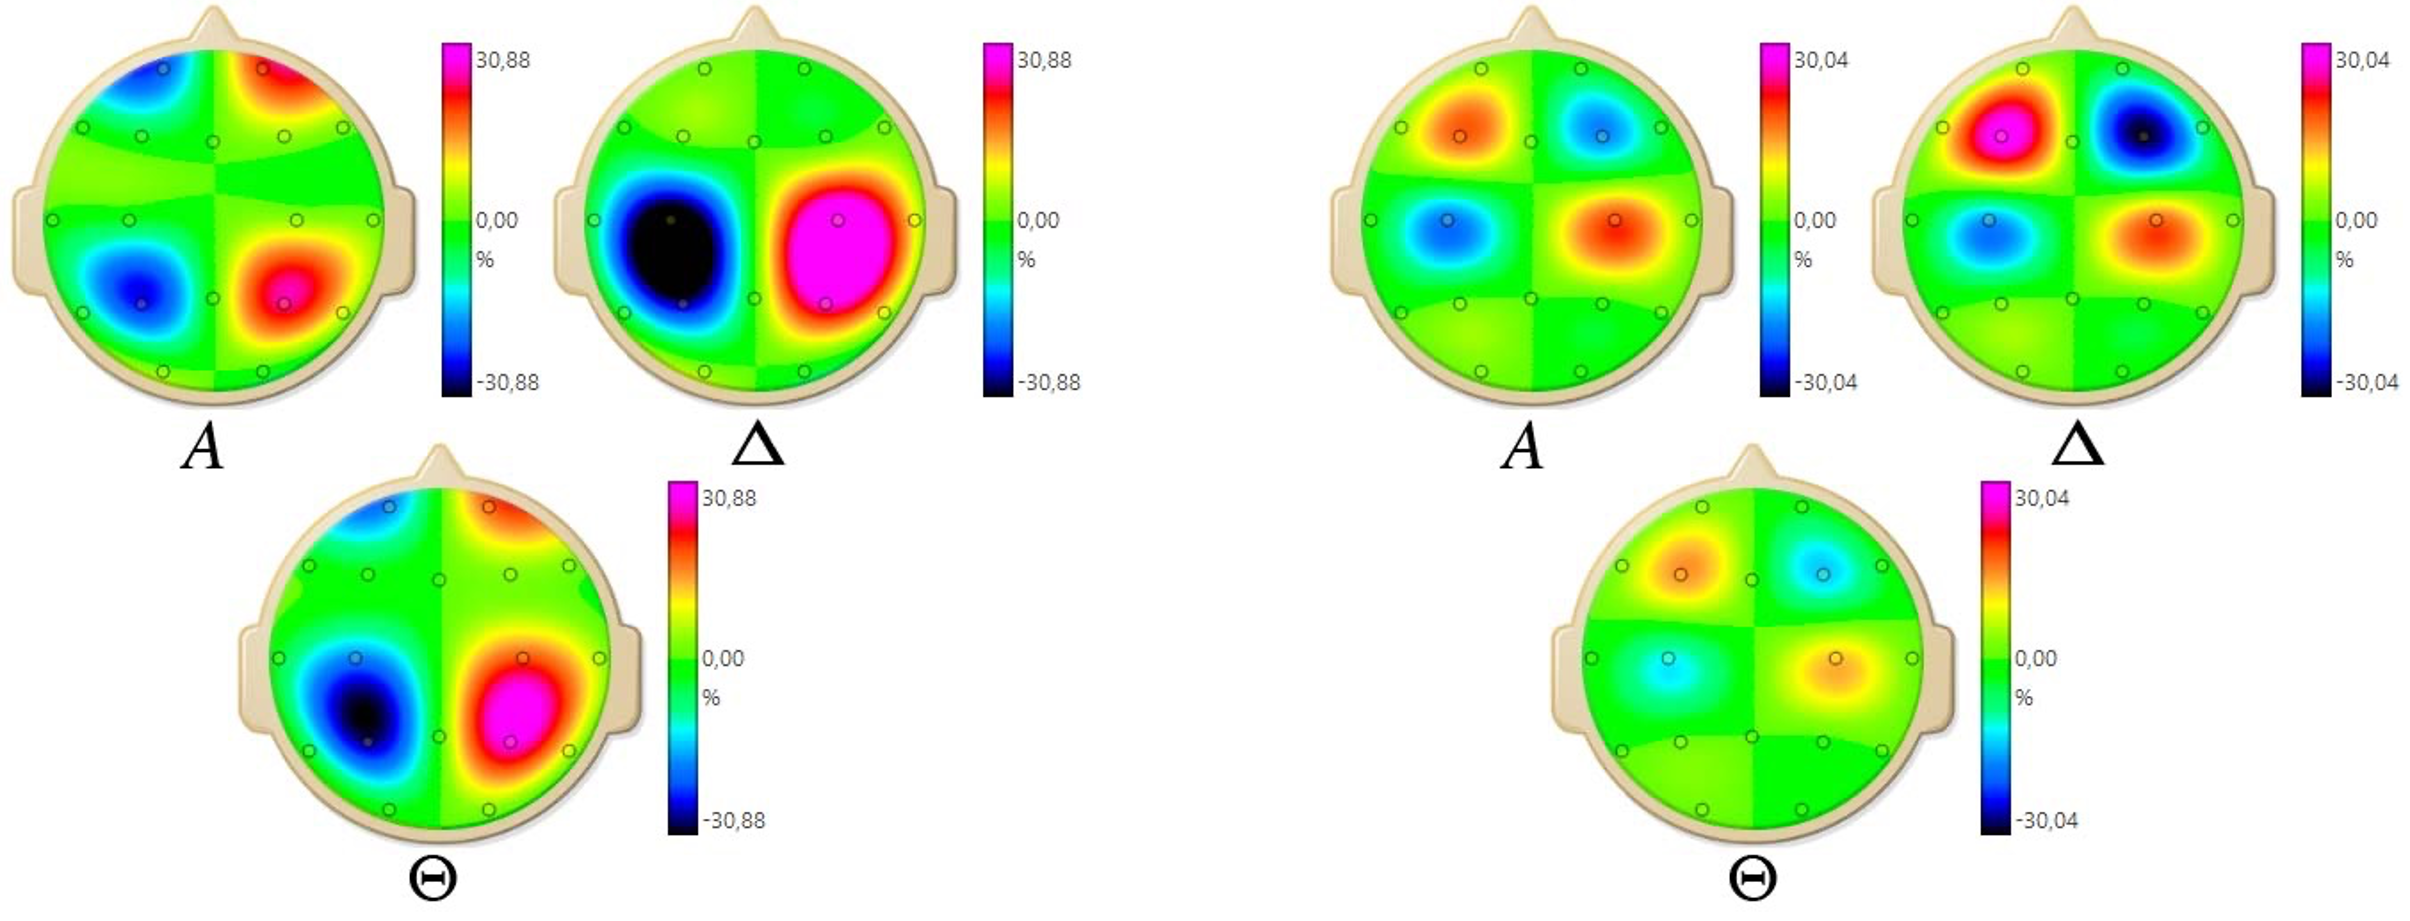
\includegraphics[width=\textwidth]{A2022.IDSEPC.ConcettoDiSoftware/SoftwareAttoCreativoEEG.png}
\end{center}

\end{frame}

\begin{frame}
{\centerline{La natura del software (2/3)}}
\begin{itemize}
    \item Il software \`{e} simile ad altri risultati di creazioni umane
\end{itemize} 
\begin{center}
    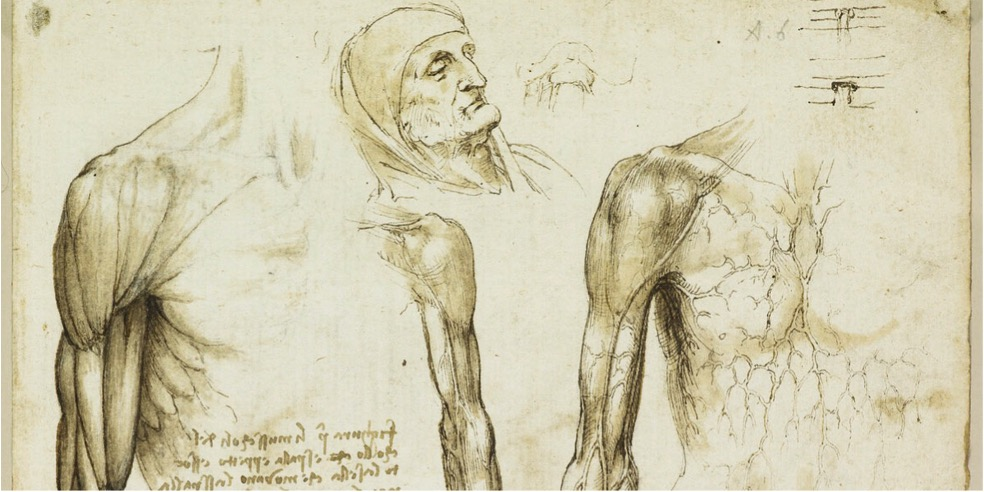
\includegraphics[width=\textwidth]{A2022.IDSEPC.ConcettoDiSoftware/SoftwareAttoCreativoLeonardo.jpg}
\end{center}

\end{frame}

\begin{frame}
{\centerline{La natura del software (3/3)}}
\begin{itemize}
    \item Il software \`{e} protetto dal diritto d'autore (anche se la questione \`{e} sempre aperta)
\begin{itemize}
    \item I diritti degli sviluppatori sono divisi in diritti morali (non alienabili) e diritti economici (alienabili)
    \item I diritti dei creatori sono protetti anche se non registrano un brevetto 
    \item I diritti durano molto pi\`{u} a lungo di quelli di un brevetto -- 50 anni dopo la morte del creatore invece che 20 anni dopo la registrazione del brevetto 
    \item Il software \`{e} dato in licenza e non venduto
\end{itemize} 
\end{itemize} 

\end{frame}

\begin{frame}
{\centerline{La funzione di costo}}
\begin{center}
    \begin{tikzpicture}[scale=0.9]
\begin{axis}[
axis x line=center,
axis y line=center,
xmin = -0.95,
xmax = 9.95,
ymin = -0.95,
ymax = 11,
title={Costo marginale per unit\`{a}},
xlabel = {Numero di unit\`{a} prodotte},
yticklabels={,,},
extra x ticks = {0},
extra x tick label = {$\hspace{-0.6cm}0$},
]
\addplot[very thick,domain=0.01:0.94,samples=100,red] {0.040*x/(ln(x)^2)};
\addplot[very thick,domain=0.94:1.06,samples=10,red] {0.040*0.94/(ln(0.94)^2)};
\addplot[very thick,domain=1.06:10,samples=100,red] {0.032*x/(ln(x)^2});
\addplot[very thick,dotted] coordinates {(1,0) (1,10)};
\addplot[thick,dashed,green] coordinates {(0,10) (10,10)};
\end{axis}
\end{tikzpicture}
\end{center}

\end{frame}

\begin{frame}
{\centerline{Esercizio proposto}}
\vspace{1cm}
\begin{center}
    \LARGE{Trovare altri settori in cui si notano funzioni di costo simili.}
\end{center}

\end{frame}


\begin{frame}
{\centerline{La segmentazione del mercato nel software}}
\begin{itemize}
\item Nel software non ci sono limiti fisici alla segmentazione
\item Inoltre:
\begin{itemize}
\item il software \`{e} protetto dal copyright
\item la funzione di costo ha una struttura a ``L''
\end{itemize}
\item Si pu\`{o} quindi operare un segmentazione aggressiva
\item Si possono operare strategie di ``bundling'' per promuovere nuovi prodotti
\end{itemize}

\end{frame}

\begin{frame}
{\centerline{Esempio di segmenti di mercato}}

\begin{itemize}
    \item Questi dati sono molto vecchi, ma il succo non cambia:
\end{itemize}

\begin{center}
    
\resizebox{0.9\textwidth}{!}{%
  \begin{tabular}{|c|c|c|c|}
  \hline
  \textbf{Prodotto} & \textbf{Professional} & \textbf{Educational} & \textbf{E/P} \\
  \hline
    Office 97 & \$ 779 & \$ 215.45 & 27.6\% \\ \hline
    Corel WP Suite 98 & \$ 449 & \$ 71.55 & 15.9\% \\
  \hline
  \end{tabular}

} % end of scope of "\resizebox"  directive
\end{center}
\end{frame}

\begin{frame}
{\centerline{Altro esempio di segmentazione (16/09/2022)}}
\begin{center}
    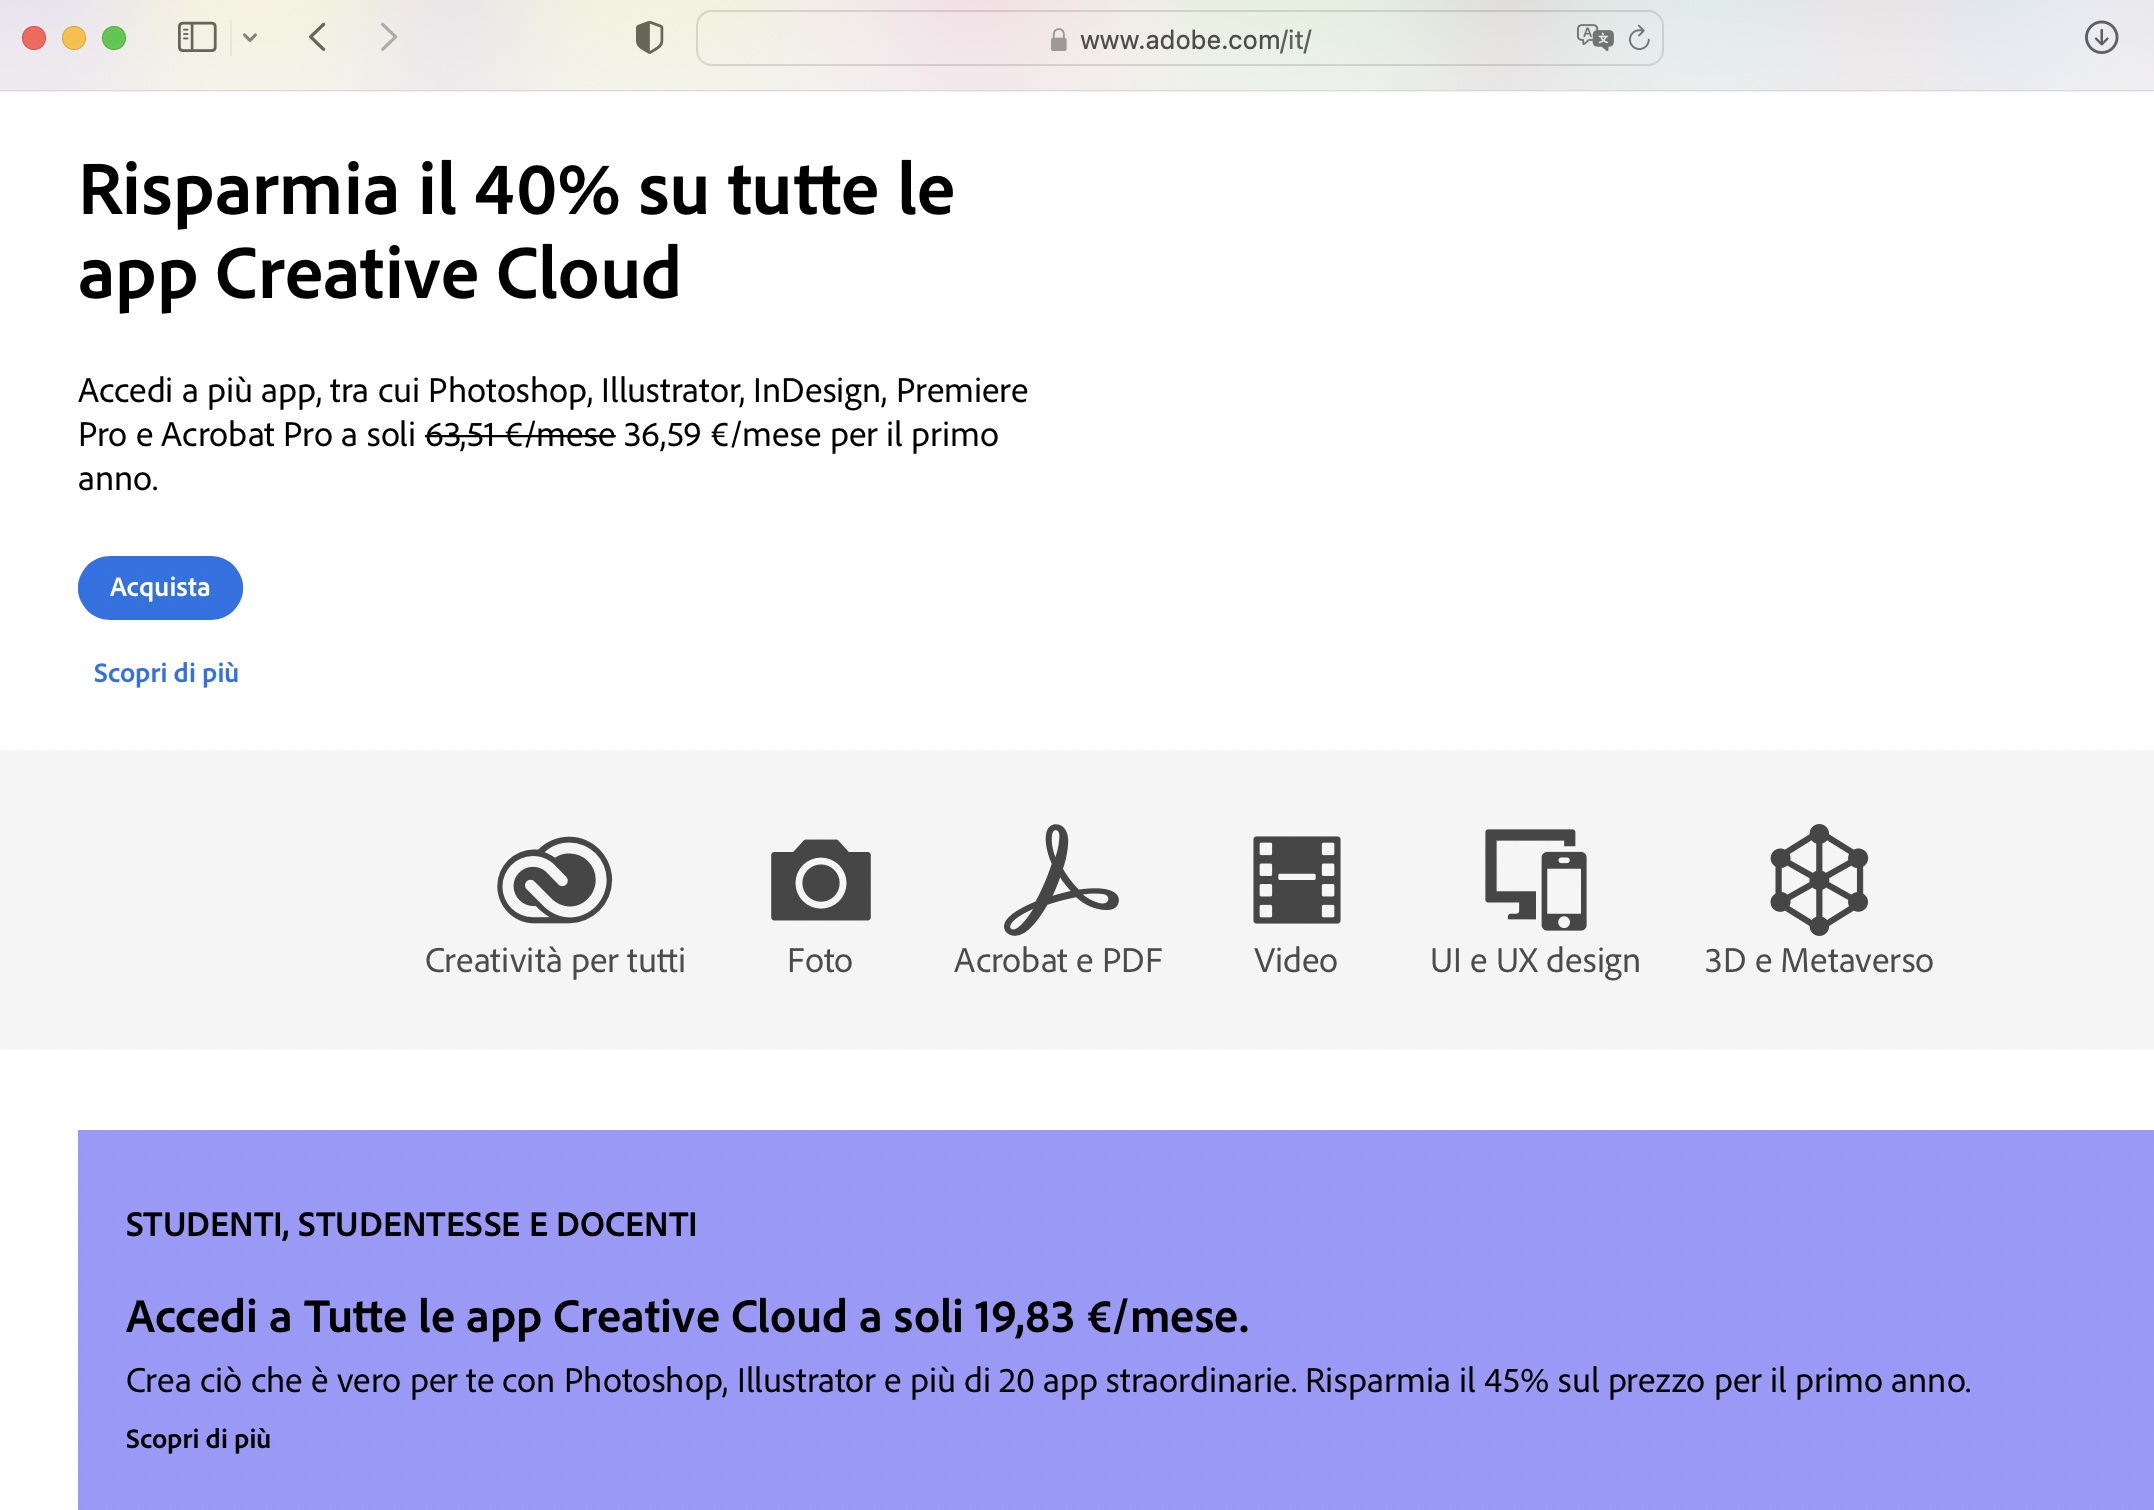
\includegraphics[width=0.8\textwidth]{A2022.IDSEPC.ConcettoDiSoftware/SegmentationBundlingAdobe.jpg}
\end{center}

\end{frame}

\begin{frame}
{\centerline{Bundling (16/09/2022)}}
\begin{center}
    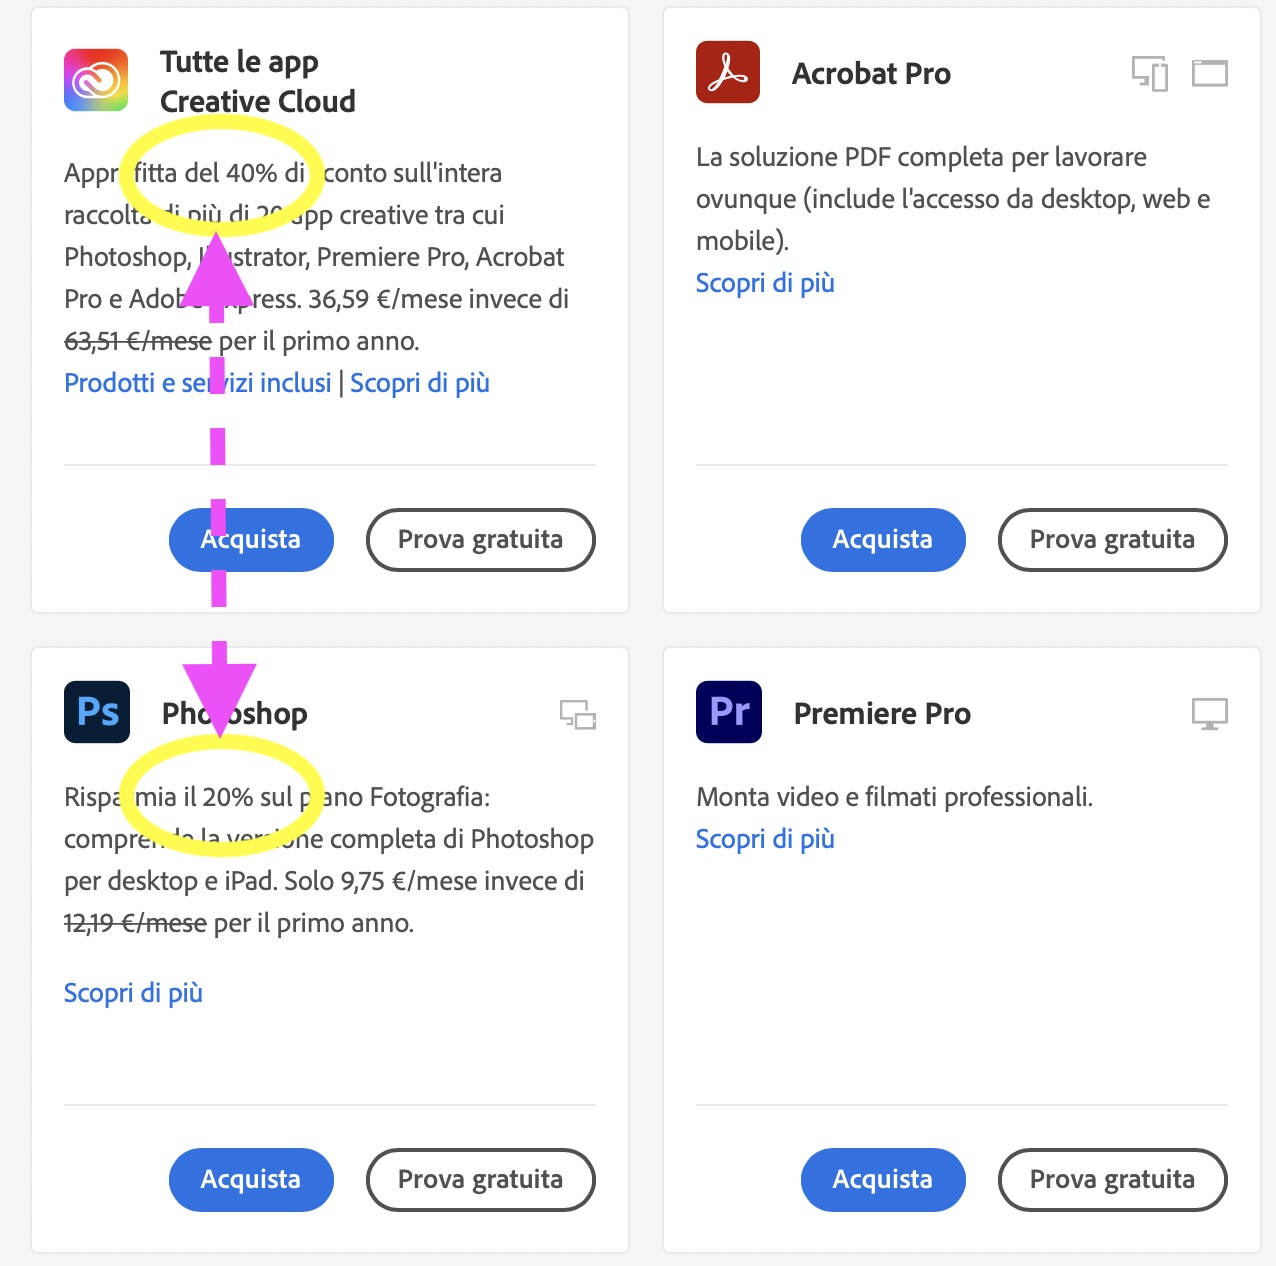
\includegraphics[width=0.6\textwidth]{A2022.IDSEPC.ConcettoDiSoftware/BundlingAdobe.jpg}
\end{center}

\end{frame}

\begin{frame}
{\centerline{Bundling in altri settori ``creativi'' (1/2)}}
\begin{center}
    
\includegraphics[width=0.4\textwidth]{A2022.IDSEPC.ConcettoDiSoftware/BundlingMarvel.pdf}
\end{center}

\end{frame}

\begin{frame}
{\centerline{Bundling in altri settori ``creativi'' (2/2)}}
\begin{center}
    
\includegraphics[width=0.45\textwidth]{A2022.IDSEPC.ConcettoDiSoftware/BundlingAD.pdf}
\end{center}

\end{frame}

\begin{frame}
{\centerline{Esercizio proposto}}
\vspace{1cm}
\begin{center}
    \LARGE{Presentare esempi di bundling sperimentati di persona.}
\end{center}

\end{frame}



\begin{frame}
{\centerline{Esternalit\`{a} di rete}}

\begin{itemize}
\item Si hanno \textcolor{blue}{economie di rete} per un prodotto quando un utente lo valuta  diversamente se ci sono utenti di tale prodotto o di prodotti \textit{compatibili}.

\item Quando il valore di un prodotto aumenta quanti pi\`{u} ci sono utenti di tale prodotto o di prodotti compatibili si dice che ci sono \textcolor{red}{esternalit\`{a} di rete}, o, semplicemente \textcolor{red}{esternalit\`{a}}.


\end{itemize}

\end{frame}

\begin{frame}
{\centerline{Esempi di esternalit\`{a} di rete}}

\begin{itemize}
\item Il mercato delle telecomunicazioni \`{e} un chiaro esempio di esternalit\`{a} di rete: 
\begin{itemize}
\item il valore di un telefono dipende da quanti utenti lo usano. Se nessuno lo usasse, sarebbe inutile!
\end{itemize}
\item Anche il mercato delle figurine Panini \`{e} un chiaro esempio di esternalit\`{a} di rete!

\item Non tutti i mercati hanno esternalit\`{a} di rete: quello delle automobili di lusso, sicuramente no:
\begin{itemize}
\item chi compera un'auto di lusso spera probilmente di essere l'unico nel suo circolo ad averla.
\end{itemize}
\item La stessa situazione si ha con i vestiti di lusso.

\end{itemize}

\end{frame}

\begin{frame}
{\centerline{Esternalit\`{a} di rete nel software}}

\begin{itemize}
\item L'industria software ha forti esternalit\`{a} di rete.
\item Ci sono due chiari esempi di tali esternalit\`{a}:
\begin{itemize}
\item lo scambio di informazioni, ad esempio via posta elettronica o tramite la condivisione di formati di file (ad esempio .docx o .odt)
\item l'usabilit\`{a} dei sistemi software, per cui se si conosce la modalit\`{a} di uso di un sistema, si tende ad usare sistemi con le stesse modalit\`{a}, ad esempio, con le stesse scorciatoie
\end{itemize}

\end{itemize}

\end{frame}

\begin{frame}
{\centerline{Esercizio proposto}}
\vspace{1cm}
\begin{center}
    \LARGE{Identificare casi di esternalit\`{a} di rete presenti nella vita di ogni giorno.}
\end{center}

\end{frame}


\begin{frame}
{\centerline{Effetti delle esternalit\`{a} di rete (1/3)}}

\begin{itemize}
\item I mercati con forti esternalit\`{a} di rete stimolano le aziende a saltare sul carro di nuove tecnologie, anche se tali tecnologie devono ancora provare la loro efficacia;
\begin{itemize}
\item questo fenomeno viene chiamato \textcolor{red}{insufficient friction} (frizione insufficiente) oppure \textcolor{blue}{excess bandwagon} (carrozzone eccessivo).
\end{itemize}

\end{itemize}

\end{frame}

\begin{frame}
{\centerline{Effetti delle esternalit\`{a} di rete (2/3)}}

\begin{itemize}
\item Le esternalit\`{a} possono produrre effetti di riduzione della fluidit\`{a} degli uteni su prodotti
\begin{itemize}
\item ci\`{o} viene chiamato \textcolor{red}{lock-in} (chiusura) e si manifesta con la presenza di \textcolor{blue}{barriere di ingresso}, ovvero la necessit\`{a} di costi aggiuntivi per passare ad altri prodotti equivalenti o equivalenti a prodotti compatibili
\end{itemize}
\item Un tipico esempio di questo è stato il formato Betamax \url{https://it.wikipedia.org/wiki/Betamax}

\end{itemize}

\end{frame}


\begin{frame}
{\centerline{Effetti delle esternalit\`{a} di rete (3/3)}}

\begin{itemize}

\item La presenza di un monopolista in un mercato ad alta tecnologia con esternalit\`{a} di rete pu\`{o} incutere paura a possibili compratori timorosi di affidarsi ad un singolo venditore in quanto:
\begin{itemize}
\item agli occhi dei potenziali compratori il mercato pu\`{o} essere considerato ancora troppo immaturo,
\item i potenziali compratori possono aver paura che il monopolista collassi o aumenti arbitrariamente i prezzi dei prodotti.
\end{itemize}

\end{itemize}

\end{frame}


\begin{frame}
{\centerline{Esercizio proposto}}
\vspace{1cm}
\begin{center}
    \LARGE{Trovare effetti delle tre esternalit\`{a} di rete nella propria esperienza.}
\end{center}

\end{frame}

\begin{frame}
{\centerline{Visualizzazione del mercato -- Valore}}
\begin{itemize}
    \item Come analizzare il valore del prodotto
\end{itemize} 
\begin{center}
    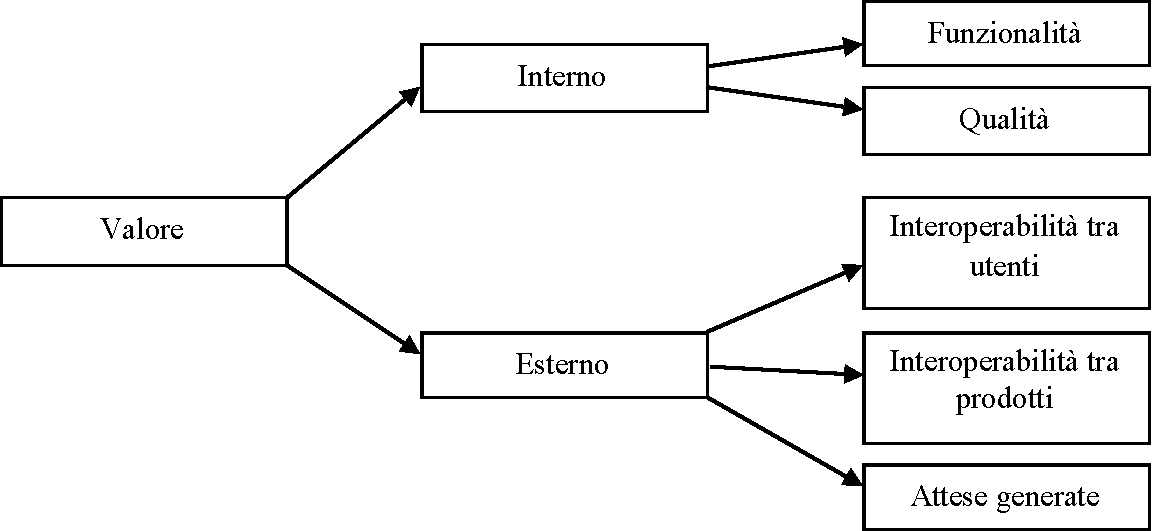
\includegraphics[width=\textwidth]{A2022.IDSEPC.ConcettoDiSoftware/ValoreDelProdotto.pdf}
\end{center}

\end{frame}

\begin{frame}
{\centerline{Visualizzazione del mercato -- Compatibilit\`{a}}}
\begin{itemize}
    \item Come analizzare la compatibilit\`{a} tra prodotti via formati dei dati
\end{itemize} 
\begin{center}
    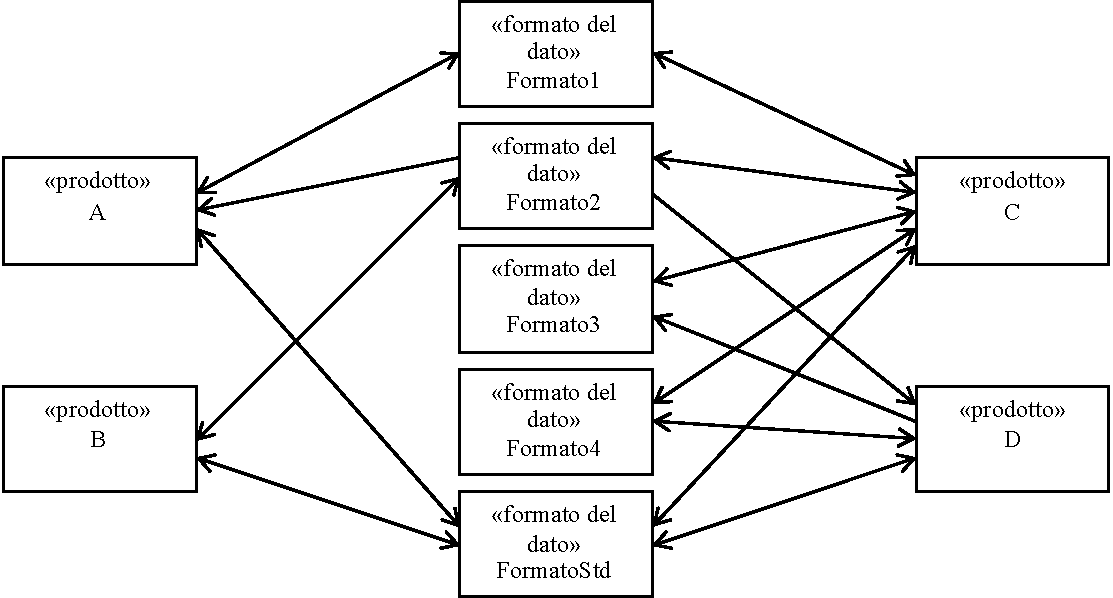
\includegraphics[width=0.9\textwidth]{A2022.IDSEPC.ConcettoDiSoftware/CompatibilitaProdotti.pdf}
\end{center}

\end{frame}
\begin{frame}
{\centerline{Esempi di compatibilit\`{a} (1/2)}}
\begin{itemize}
    \item Esempio di come presentare le compatibilit\`{a} per Word
\end{itemize} 
\begin{center}
    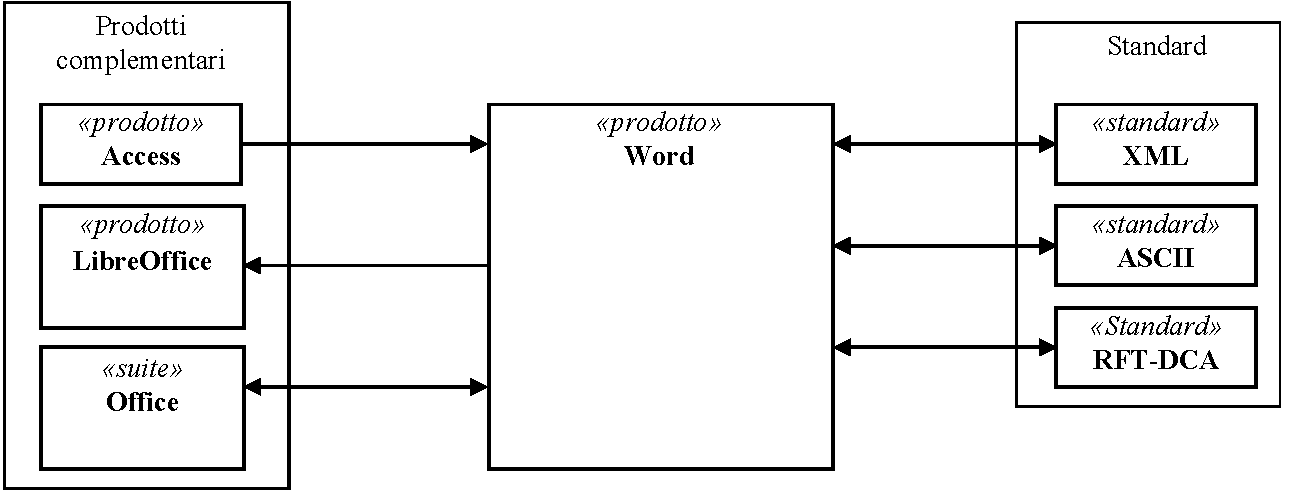
\includegraphics[width=0.9\textwidth]{A2022.IDSEPC.ConcettoDiSoftware/EsempiCompatibilita.1.pdf}
\end{center}

\end{frame}

\begin{frame}
{\centerline{Esempi di compatibilit\`{a} (2/2)}}
\begin{itemize}
    \item Esempio di come presentare le compatibilit\`{a} per Word
\end{itemize} 
\begin{center}
    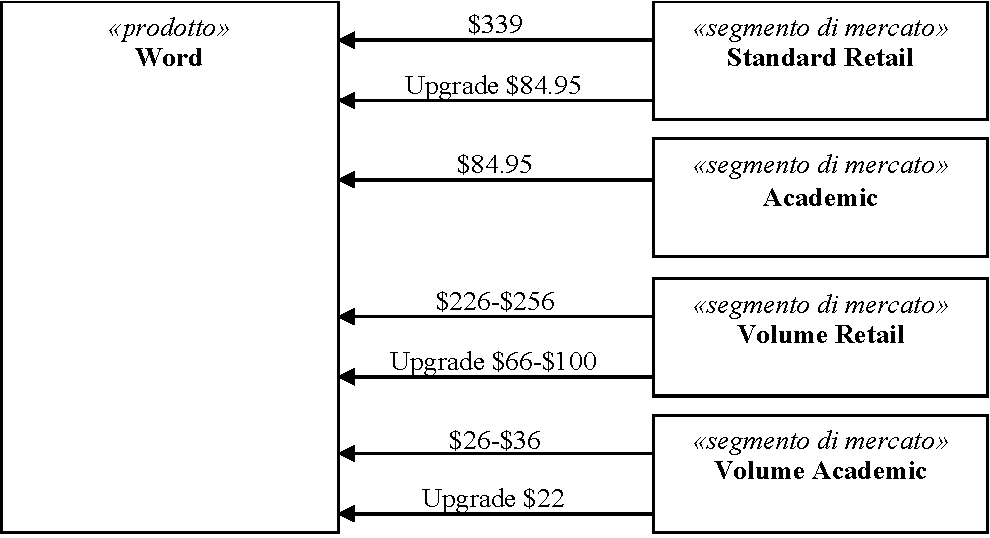
\includegraphics[width=0.9\textwidth]{A2022.IDSEPC.ConcettoDiSoftware/EsempiCompatibilita.2.pdf}
\end{center}

\end{frame}

\begin{frame}
{\centerline{Esercizio proposto}}
\vspace{1cm}
\begin{center}
    \LARGE{Tracciare il diagramma di compatibilit\`{a} per un prodotto soggetto a esternalit\`{a} a vostra scelta.}
\end{center}

\end{frame}


\begin{frame}
{\centerline{Strategie comunemente utilizzate}}

\begin{itemize}
    \item Upgrade di prodotti
    \item Upgrade competitivi
    \item Suite di prodotti
\end{itemize}

\vspace{1cm}
\begin{center}
    
\resizebox{0.9\textwidth}{!}{%
  \begin{tabular}{|c|c|c|c|}
  \hline
  \textbf{Strategia} & \textbf{Esternalit\`{a}} & \textbf{Bundling} & \textbf{Segmentazione} \\
  \hline
    Upgrade di prodotti & $\times$ &  -- & $\times$ \\ \hline
    Upgrade competitivi & $\times$ & -- & $\times$ \\ \hline
    Suite di prodotti & $\times$ & $\times$ & -- \\
  \hline
  \end{tabular}

} % end of scope of "\resizebox"  directive
\end{center}

\end{frame}

\begin{frame}
{\centerline{Esercizio proposto}}
\vspace{1cm}
\begin{center}
    \LARGE{Identificare strategie presenti nel prodotto soggetto a esternalit\`{a} da voi precedentemente prescelto.}
\end{center}

\end{frame}


\begin{frame}
{\centerline{Domande?}}
\vspace{1cm}
\begin{center}
    \LARGE{Fine della seconda lezione.}
\end{center}

\end{frame}


\end{document}
